\documentclass[11pt]{article}

\marginparwidth 0.5in 
\oddsidemargin 0.25in 
\evensidemargin 0.25in 
\marginparsep 0.25in
\topmargin 0.25in 
\textwidth=6in
\textheight=8in

\usepackage{indentfirst}
\usepackage{graphicx}
\usepackage{subcaption}
\usepackage{pgffor}
\usepackage{hyperref}
\usepackage{amsmath}
\usepackage{amssymb}

\begin{document}
\hfill\vbox{\hbox{Jude Shin}
		\hbox{CSC 4888-S01}	
		\hbox{HW 4}	
		\hbox{\today}}\par

\bigskip
\centerline{\Large\bf Visual Odometry: KITTI Stereo}\par
\bigskip

\section{Explanation}

\subsection{Visual Odometry Block}

The Visual Odometry loops through all of the image pairs, treating each pair as one step in time.
Each pair of images finds keypoints.
Using those keypoints, we are able to get epipolar lines between the left and right images at that timeframe.
The algorithm loops through all images sequentially, so I keep track of the previous 3D reconstruction points and the previous descriptors.
We use those to generate a transformation matrix that holds rotation and translation between the two time steps.
This inverse translation is applied by multiplying the previous pose by the transformation matrix.
We save this pose and continue till all of the images are processed.

I just assumed the starting odometry to be $(0, 0, 0)$ to make things easy.

To find the epipolar line, I decided to not only use the constraint that each matching keypoint's difference in {\tt y} had to be $==0.0$, but that the disparity had to be $> 0.0$.
Since we know the right camera will always create a positive disparity in relation to the left camera, we can add this sanity check to make sure nothing funky is going on when calculating the epipolar lines.
I don't really know if it made any difference, but it was just adding one line of code, so I was fine with it.

I added a global constant that will skip every other {\tt EVERY\_OTHER} images and ground truths.
This allowed me to shrink the time it took to get a full picture of the odometry and debug faster.
However, this came with some side effects.
If the skip constant {\tt EVERY\_OTHER} was too big, then the function {\tt solvePnPRansac} sometimes couldn't find good rotation and translation values.
This resulted in way more drift.
Because of this, I utilized the {\tt success} flag; if {\tt solvePnPRansac} succeeded, then the algorithm would go on as normal.
If it did not succeed, then that image pair was essentially ``skipped" and the previous odometry pose was just copied to the current timeframe.
This theoretically made the algorithm continue to work, even when the translation matrix could not be found.
I started seeing noticeable issues when {\tt EVERY\_OTHER} was greater than 5.
I think it had a hard time when the skipped images covered a corner change.

\subsection{Plotting Block}

This code is almost identical to all of the plotting functions that we have done for previous homework assignments and labs in this course.
It takes only the x and z locations in both the computed odometry locations and the given ground truth dataset.

\section{Discussion Questions}

\begin{enumerate}
	\item The error in the Visual Odometry estimate increases over time - this is called  ``drift".
		Why does this occur?

		{\it Drift occurs because not every estimate is perfect. 
		Each estimate is calculated based on previous estimates.
		Over time, the error accumulates to a noticeable amount.}

	\item Describe some ideas for how to reduce drift in the Visual Odometry estimate.

		{\it Taking more images will produce less accumulated error.
		I tried taking every other image in the dataset, there seemed to be a lot more drift.
		I even tried skipping every 5 images, and sometimes the {\tt solvePnPRansac} function failed to produce a good transformation matrix.}

		{\it Another way to get more data would be to add more cameras.
		Another stereo pair of images could give us another estimate of the 3d camera location.
		Then we could average the results against the two.}

		{\it I think adding a threshold for the epipolar mask would actually do more good than harm.
		Intuitively it seems like increasing the margin for error would give us worse results, but increasing this tolerance will increase the number of keypoints that we can use.
		The more keypoints are more important as we can triangulate more, getting a better average on the real-world 3D point.
		The run that used a strict epipolar constraint of $==0.0$ (Figure~\ref{fig:no_thresh}) seems to be slightly more off course at the end in comparison to the run that used a epipolar constraint of $<=1.0$ (Figure~\ref{fig:thresh}).}

\end{enumerate}

\begin{figure}[h!]
	\centering
	\begin{minipage}{0.45\textwidth}
		\centering
		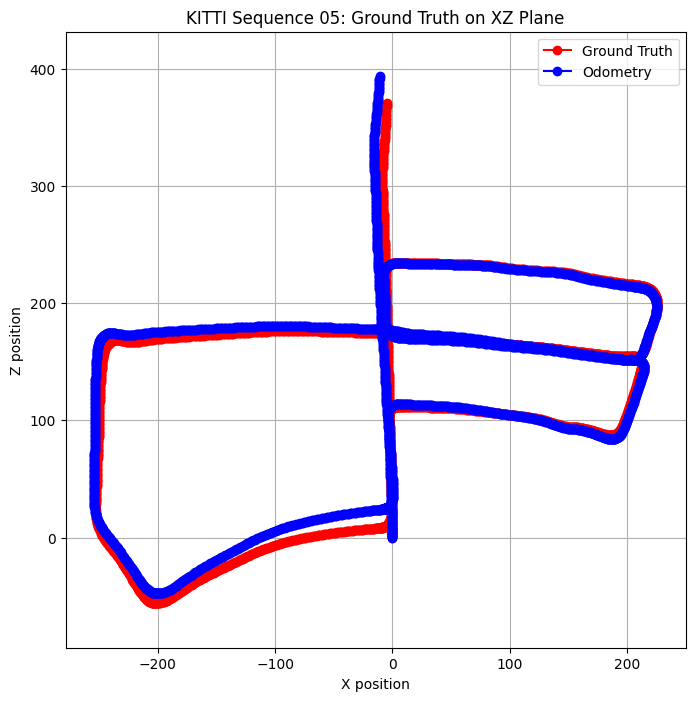
\includegraphics[width=\textwidth]{assets/no_thresh_01.png}
		\caption{Odometry results without a threshold (Epipolar mask: $==0.0$).}
		\label{fig:no_thresh}
	\end{minipage}
	\hfill
	\begin{minipage}{0.45\textwidth}
		\centering
		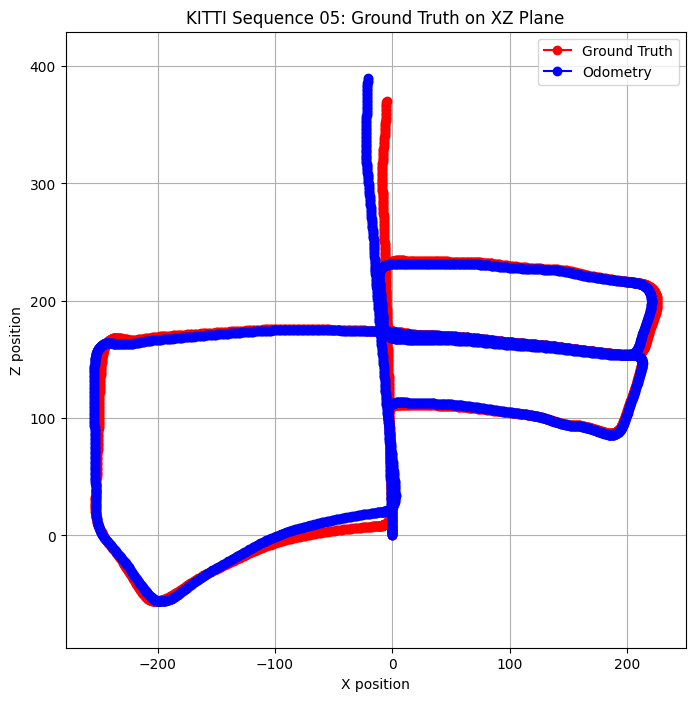
\includegraphics[width=\textwidth]{assets/thresh_01.png}
		\caption{Odometry results with a threshold (Epipolar mask: $<=1.0$).}
		\label{fig:thresh}
	\end{minipage}
\end{figure}

\clearpage

\section{Sources Used}

The \href{https://docs.opencv.org/5.0/}{cv2 docs} and \href{https://numpy.org/doc/}{numpy docs} were used to look up examples and the use of functions like {\tt cv2.solvePnPRansac}, {\tt cv2.triangulatePoints}, {\tt np.linalg.inv}, and {\tt np.matmul}.

I had to look up some implementation to get a rotation matrix from the rotation vector given from {\tt cv2.solvePnPRansac}.
Thankfully there was a function documented \href{https://docs.scipy.org/doc/scipy/reference/generated/scipy.spatial.transform.Rotation.from_rotvec.html}{here}.
It honestly would have been faster to just hardcode the 3x3 matrix from the slides, but it is what it is.

\end{document}
